\documentclass[22pt]{beamer}
\usepackage[orientation=portrait, size=custom, width=91.44, height=91.44,scale=1.2]{beamerposter} % 36in*2.5 = 90cm
\usepackage[absolute,overlay]{textpos}
\usepackage{bookmark} %pdflatex says to use this to avoid errors...
\usepackage{graphicx} %for including images
\graphicspath{{figs/}} %location of images
\usepackage{wrapfig} %wrap text around the images
\usepackage{listingsutf8}    %package for code environment; use this instead of verbatim to get automatic line break; use this instead of listings to get (•)
\usepackage{amsmath}
\usepackage{gensymb}
\usepackage[export]{adjustbox}
\usepackage[skins,theorems]{tcolorbox}
\usepackage{tikz}
\newcommand*\circled[1]{\tikz[baseline=(char.base)]{
            \node[shape=circle,draw,inner sep=2pt] (char) {#1};}}
\usepackage{array}
\usepackage{booktabs,adjustbox}
\usepackage{subcaption}
\usepackage{pgfplots}
%plot options
\pgfplotsset{width=7cm,compat=1.8}
\PassOptionsToPackage{gray}{xcolor}

\usetikzlibrary{shapes,shapes.geometric,arrows,fit,calc,positioning,automata,}

\usepackage{wrapfig}

%\mode<presentation>
%this doesn't seem to make any difference; leave for now for trying out
\usetheme{Berlin}
\definecolor{MacBlue}{rgb}{0.10196,0.22353,0.53725}
\definecolor{MacMaroon} {rgb}{0.47843, 0, 0.23137}
\definecolor{MacMaroon2} {rgb}{0.47451, 0, 0}
\definecolor{MacGray}{rgb}{0.50196,0.49804,0.51765}
\definecolor{MacMaroon3}{rgb}{00.47,0.2,0.31}
\definecolor{MacGold}{rgb}{1, 0.75,0.35}
\usecolortheme[named=MacMaroon2]{structure}
\setbeamertemplate{caption}[numbered]
\setbeamertemplate{navigation symbols}{}

\title{HubListener: Software Metrics Analysis \& Modelling for Open-Source Projects on Github }
\subtitle{}  %probably want a better subtitle
  \author[Zed Ahmad, Prakhar Jalan, Pedro Oliveira \& Piranaven Selvathayabaran]{Zed Ahmad, Prakhar Jalan, Pedro Oliveira, Piranaven Selvathayabaran \newline supervised by Dr.~Spencer Smith$^\dagger$ \vspace{0.3cm}}
  \institute[McMaster University]{$^\dagger$Department of Computing and Software, McMaster University

1280 Main St. W, Hamilton, Ontario, Canada L8S 4L8}
  \date{December 5th, 2018}

\begin{document}
%compile with pdflatex

%there is only one frame, because there is only one page; yeah, it's a poster
%textblock and block seem to work nicely to organize layout
\begin{frame}[fragile]

\begin{textblock}{2}(0.7,1)

\includegraphics[height=8.5cm]{englogo.png} % We can use CAS logo as well? 
\end{textblock}

\begin{textblock}{2}(12.7,0.80)

\includegraphics[height=10.5cm]{caslogo.png} 
\end{textblock}

\begin{textblock}{8}(4,1)
\titlepage
\end{textblock}

\begin{textblock}{7.25}(0.5,3.1)
\begin{block}{Project Purpose}
The HubListener tool was designed to provide users with relevant metrics, trends, and information regarding their GitHub projects. The goal here is to bring this set of organized data to the user’s attention and push them to make any improvements or corrections; as a means of project review and evaluation. Our tool puts a given repository against a set of the most popular projects on GitHub, making comparisons wherever possible. This however begs the question, “What specific metrics lead to success, and how do we measure this success?”
\end{block}

\begin{block}{Target Users}
The HubListener Tool's general consumer audience would be any member of the open-source community. We have however specifically targetted those with expertise using open-source software. As seen in the 'Proof of Concept' section, a friendly user interface has not yet been implemented, and so the user should at least be familiar with the use of a Command Line Interface.
\newline
\newline
Example User Groups:
\begin{itemize}
\item Developers and Creators 
\item Students (i.e. Engineers)
\item Researchers
\item Companies/Organizations
\end{itemize}
\end{block}

\begin{block}{Proof of Concept}
\begin{figure}
  \begin{subfigure}{0.96\textwidth}
    \centering
     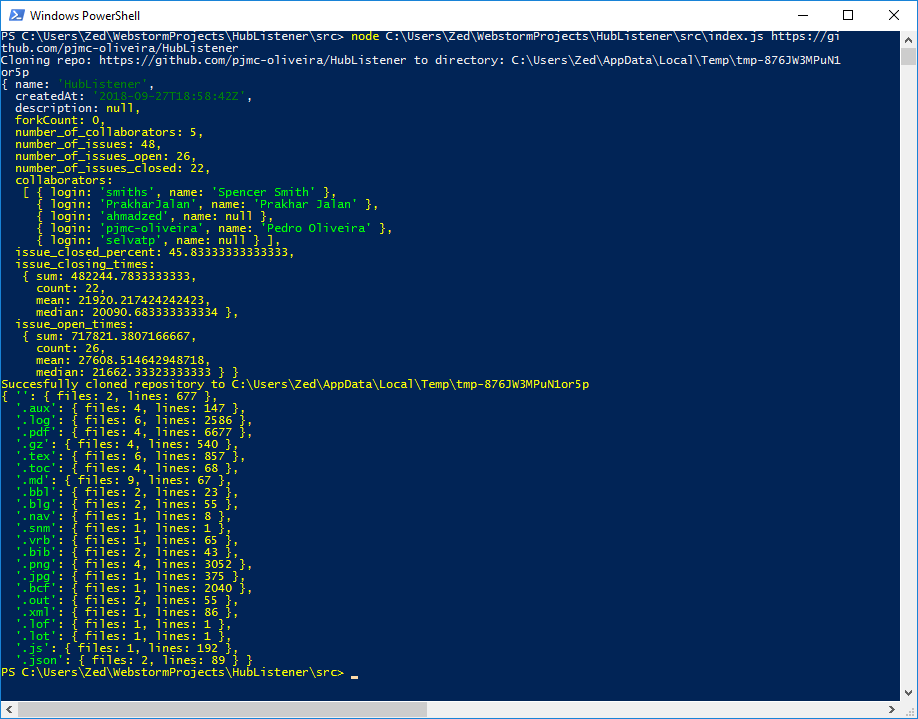
\includegraphics[width=39cm]{PowerShellPOC.png} 
  \end{subfigure}
\end{figure}
The user enters the project URL via the Command Line Interface, and is provided the output in an array. This output consists of a large list of metrics that are pulled directly from GitHub.

\end{block}

\end{textblock}

\begin{textblock}{7.25}(8.25,3.1)
\begin{block}{Output of Metrics}
The user provides the GitHub repository link as input, and we return the following output and more:
\begin{itemize}
\item Cyclomatic Complexity 
\item Essential Complexity 
\item Integration Complexity 
\item Cyclomatic Density
\item Lines of Code 
\item Lines of Comments 
\item Maintainability Index 
\item Coupling Metric 
\item Number of Methods
\item Number of Variables 
\item Number of Issues 
\item Number of Bugs 
\item Number of Stars 
\item Functional Coverage Score
\item Condition Coverage Score 
\end{itemize}

Below are some examples of trends that can be viewed via GitHub. However, our goal is to provide a trend pairing any of the metrics jotted above (or observe the pattern across time), as GitHub is unable to do so currently. 

\begin{figure}
  \begin{subfigure}{0.40\textwidth}
    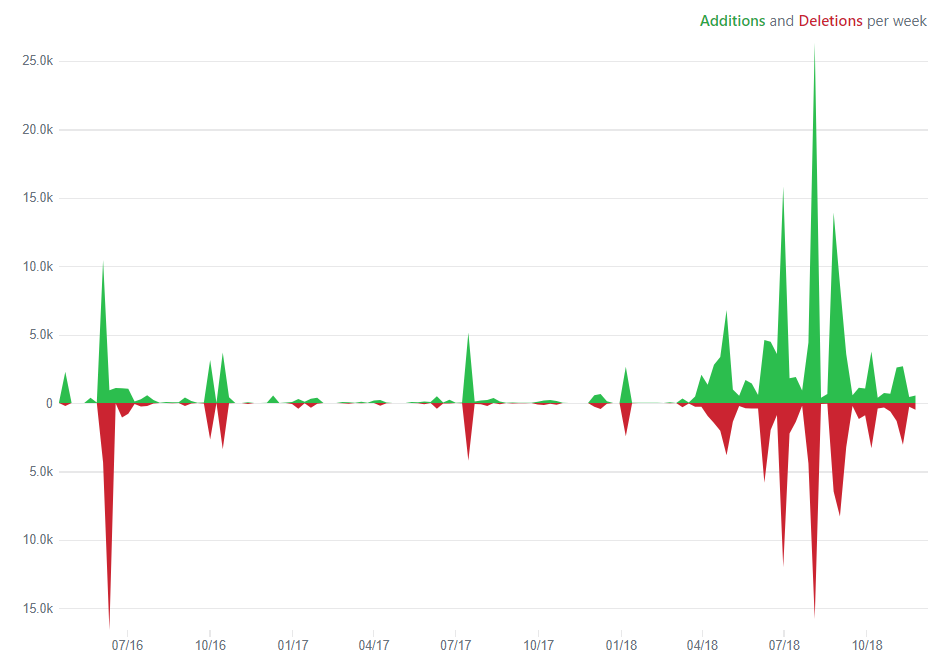
\includegraphics[height=11cm]{AddDeleteVisual1.png}
        \caption*{Example 1: A visualization of additions and deletions from a GitHub repository. }
  \end{subfigure}
  \begin{subfigure}{0.40\textwidth}
    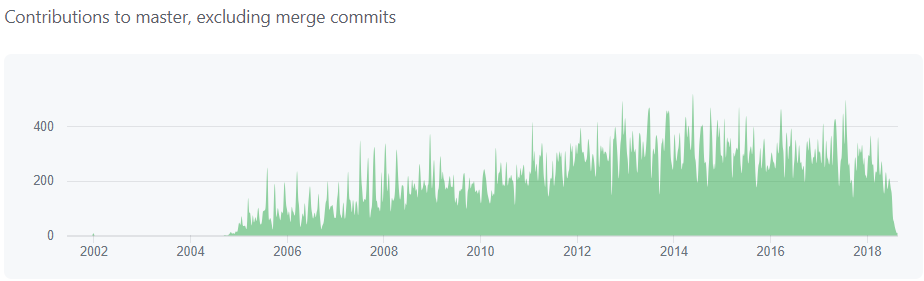
\includegraphics[height=12cm, width = 18cm]{Contributions.png}
        \caption*{Example 2: A visualization of contributions to a repository over time. }
    \end{subfigure}
 \end{figure}

\end{block}

\begin{block}{Project Goals \& Future Work}
We hope that our tool will provide valuable metrics or trends to at least 20 users, leading to any changes (minor or major) to their GitHub project; at which point our team can safely say that we have succeeded with this project. Future work includes creating a friendly user interface for easier use of our application, as well as expanding the amount of metrics and trends analyzed. We also wish to add more user options/customizability, so that they are able to be more selective when it comes to the output of HubListener.
\end{block}

\begin{block}{Acknowledgements}
The HubListener Capstone team would like to thank Dr. Smith for supervising this project. Our shared enthusiasm for this project, along with his consistent input, has been instrumental to our ongoing success. We would also like to thank Dr. Anand for his organization of the course and the Faculty of Engineering at McMaster for providing us the platform to pursue a project of this magnitude. We greatly appreciate all the feedback the students, faculty and staff have provided on this project. Your comments and concerns continue to fuel our passion for HubListener. 
\end{block}


\begin{block}{References}
\setbeamertemplate{bibliography item}{\insertbiblabel}
\bibliographystyle{ieeetr}
{\scriptsize
\bibliography{bib}}
\end{block}



\begin{comment}
%these aren't in any particular style, it's just the basic idea
\begin{block}{References}
\setbeamertemplate{bibliography item}{\insertbiblabel}
\bibliographystyle{ieeetr}
{\scriptsize
\bibliography{bib}}
\end{block}
\vspace{-1.8mm}
%will need some more graphics to thank the various people
\end{comment}
\begin{figure}[htbp]
\end{figure}
\end{textblock}


\end{frame}
\end{document}
